\documentclass[a4paper, 12pt]{book}

\usepackage{graphicx}
\usepackage[utf8x]{inputenc}
\usepackage[T1]{fontenc}

\begin{document}

\chapter{Pruebas y Códigos de ejemplo}
Para comprobar que la aplicación satisface todos los objetivos establecidos, y que los realiza de forma correcta, se somete a una serie de 
pruebas para determinar su fiabilidad y consistencia. En base a dichas pruebas, se realizan las pertinentes correcciones hasta obtener un sistema
completamente depurado y de calidad.

Dividiremos las pruebas en dos tipos:

\begin{itemize}
 \item Pruebas sobre el funcionamiento de la interfaz.
 \item Pruebas de ejecución.
\end{itemize}


\section{Pruebas sobre el funcionamiento de la interfaz}
Tal y como indica el título de este apartado, se realizarán pruebas sobre los distintos elementos de la interfaz, las cuáles se irán describiendo
en las diferentes secciones presentadas a continuación.

\subsection{Visualización de opciones}
A continuación se detallarán las pruebas en relación a la correcta visualización de los distintos elementos de la interfaz, así como los errores 
encontrados y las soluciones aportadas. Se contemplan los siguientes casos:

\begin{itemize}
  \item Visualización de los distintos apartados y subapartados (si procede) de la barra de menú.
  \item Visualización de los distintos iconos que forman la barra de herramientas.
  \item Actualización de la información de la barra de estados.
  \item Visualización de información al dejar el cursor sobre un botón.
  \item Coloreado de palabras reservadas del lenguaje Sticky.
\end{itemize}

Se ha comprobado que, al hacer click en cualquier elemento principal del menú, se muestra el listado de acciones disponibles para cada sección.
Además, al pasar el ratón por dichas opciones, se puede observar como cambia la información de la barra de estado.

Por otra parte, podemos observar como aparece cierta información al dejar el ratón sobre cualquier botón de la barra de herramientas, la cuál
es coherente con respecto a la imagen mostrada.

Finalmente, también se ha comprobado que al escribir palabras reservadas de nuestro lenguaje, como pueden ser "mientras", "var" o "mover", se
muestran en azul, color elegido para dicho fin.

\subsubsection*{Problemas encontrados}

\begin{enumerate}
  \item La ventana de la aplicación se salía de los márgenes dependiendo del equipo en el que se estuviese usando.
  \item Se han encontrado palabras reservadas del lenguaje que no se definían como tal, es decir, no se mostraban en azul.
\end{enumerate}

\subsubsection*{Soluciones aplicadas}

\begin{enumerate}
  \item Se ha reajustado la ventana a una resolución óptima.
  \item Se han enumerado el conjunto de palabras que no se mostraban correctamente y se ha modificado el código oportuno.
\end{enumerate}

\subsection{Ejecución de opciones}
En este apartado se han puesto a prueba los diferentes elementos de la barra de menú y los botones de la barra de herramientas. En esta ocasión
se han tenido en cuenta los siguientes casos:

\begin{itemize}
  \item Funcionamiento de botones de la barra de herramientas.
  \item Ejecución de las distintas opciones de la barra de menús.
  \item Comprobación de funcionamiento de los atajos de teclado.
\end{itemize}

En primer lugar, atendiendo a las opciones del menú podemos afirmar que funcionan a la perfección, tanto al hacer click en las mismas como al
usar los atajos de teclado proporcionados, los cuáles aparecen mostrados justo en el lado derecho de la opción. Por lo tando, si tomamos como ejemplo la opción 
de deshacer código, similar a la de cualquier editor, se ejecutará tanto al realizar la acción "Edición -> Deshacer" como al pulsar "Control+Z".
Además, se ha comprobado que los botones, uno a uno, realizan su cometido de forma correcta y rápida.

\subsubsection*{Problemas encontrados}

\begin{enumerate}
  \item Nos hemos encontrado con opciones, tanto el la barra de menús como de herramientas, que no realizaban las acciones que se les requería.
	Por ejemplo, al elegir un nivel de depuración 0, no mostraba únicamente los errores producidos, sino que también mostraba otra información
	adicional que correspondía a otro nivel.
  \item En ocasiones, al ejecutar codigo inestable, no se informaba del error en el resultado de la interpretación. Un ejemplo ha sido al intentar
	hacer una conversión de un String a un Double o Integer en el lenguaje Sticky.
  \item Botones que realizaban s función únicamente de forma parcial. Por ejemplo, el botón que permite interpretar el código sólo realizaba su
	tarea la primera vez que se presionaba.
\end{enumerate}

\subsubsection*{Soluciones aplicadas}

\begin{enumerate}
  \item Se ha localizado el origen del error y se ha vuelto a codificar. Finalmente, se comprobaba que realmente la acción requerida era la acción
	que se realizaba.
  \item En este caso se ha analizado el código y se han capturado las excepciones necesarias para que el error sea mostrado en el apartado de la 
	interfaz "Resultado interpretación".
  \item Tomando el ejemplo anterior, se comprobó la codificación y ahora la ventana de animación se reinicia al interpretar un nuevo codigo.
\end{enumerate}

\section{Pruebas sobre la ejecución de los ejemplos}

\subsection{Ejemplos base de la gramática}

\begin{itemize}
  
\item Declaración de variables, incremento e impresión\\

  
  A continuación se muestra un ejemplo de declaración de variables, incremento e impresión en pantalla. \\
  
  
\begin{verbatim}
var pepe= 2;
pepe++;
mostrar("Este es el valor de la variable pepe: "+pepe);
var pepe = VERDAD;
pepe = FALSO Y (VERDAD O VERDAD);
pepe = FALSO Y VERDAD O VERDAD;
$
\end{verbatim}
  
  
  
\begin{itemize}
\item Salida (Nivel de Debug 0 $\rightarrow$ Errores)
\end{itemize}
\begin{verbatim}
...INICIANDO STICKY...
Este es el valor de la variable pepe: 3
ERROR: Linea 5: Variable "pepe" no ha sido declarada, ya existe
ERROR: En línea 7 : expecting FIN_INTERPRETE, found 'null'
...FINALIZANDO STICKY...
\end{verbatim}




\item Precedencia de operaciones y operador NO\\
  

  En este ejemplo se hará hincapié en el orden de precedencia de los operadores. \\
  
  
\begin{verbatim}
var david = 2;
var prueba = NO david + 2 == 2+2 Y (FALSO O VERDAD);
var prueba2 = NO VERDAD Y FALSO; //Tiene prioridad el NO
sup prueba2;
$
\end{verbatim}
  
  
  
  \begin{itemize}
  \item Salida (Nivel de Debug 1 $\rightarrow$ Información básica)
  \end{itemize}
\begin{verbatim}
...INICIANDO STICKY...
DEBUG 1: Linea 2: Variable "pepe" ha sido declarada con valor 2
Este es el valor de la variable pepe: 3
ERROR: Linea 5: Variable "pepe" no ha sido declarada, ya existe
DEBUG 1: Linea 6: Asignacion a la variable "pepe": false
DEBUG 1: Linea 7: Asignacion a la variable "pepe": true
...FINALIZANDO STICKY...
\end{verbatim}
  
  
  
  
\item Precedencia de operaciones y operador XO\\
  
  
  Este ejemplo es parecido al anterior pero esta vez se centrará más en el operador lógico del OR exclusivo.
  
  
\begin{verbatim}
prueba = VERDAD OX (FALSO O VERDAD);
$
\end{verbatim}

  
  \begin{itemize}
  \item Salida (Nivel de Debug 1 $\rightarrow$ Información básica)
  \end{itemize}
\begin{verbatim}
...INICIANDO STICKY...
DEBUG 1: Linea 2: Variable "prueba" ha sido declarada con valor false
...FINALIZANDO STICKY...
\end{verbatim}
  
  
  
  
\item Algunos errores\\
  

  Aquí se mostrará como el sistema se comporta cuando se producen algunos errores como divisiones por cero, operaciones aritméticas con cadenas o booleanos. \\
  
  
\begin{verbatim}
var otra = pepe/0;
otra = VERDAD + 3;
otra = 3+2 Y 4>2;
var cadena = "mi cadena";
cadena = cadena +2;
$
\end{verbatim}
  
  
  
  \begin{itemize}
  \item Salida (Nivel de Debug 0 $\rightarrow$ Errores)
\end{itemize}
\begin{verbatim}
...INICIANDO STICKY...
ERROR: Linea 3: División por 0
ERROR: Linea 4: No se pueden realizar operaciones aritméticas con valores booleanos
ERROR: Linea 5: Sólo se pueden realizar operaciones lógicas con booleanos.
ERROR: Linea 7: No se pueden realizar operaciones aritmeticas con cadenas de caracteres
...FINALIZANDO STICKY...
\end{verbatim}




\item Prueba de raíz cuadrada y potencia\\

  
  Aquí se comprobará la precedencia de operaciones en la realización de raices cuadradas y potenciaciones. \\
  
  
\begin{verbatim}
var hola; 
hola = raiz 6 + 3;
hola = raiz(6+3);
hola = 2^(-4);
hola = raiz (7^1+2);
hola = raiz 7^2+2;
hola = raiz 7^1+2;
$
\end{verbatim}
  
  

  \begin{itemize}
  \item Salida (Nivel de Debug 1 $\rightarrow$ Información básica)
  \end{itemize}
\begin{verbatim}
...INICIANDO STICKY...
DEBUG 1: Linea 2: Variable "hola" ha sido declarada
DEBUG 1: Linea 3: Asignacion a la variable "hola": 5.449489742783178
DEBUG 1: Linea 4: Asignacion a la variable "hola": 3.0
DEBUG 1: Linea 5: Asignacion a la variable "hola": 0.0625
DEBUG 1: Linea 6: Asignacion a la variable "hola": 3.0
DEBUG 1: Linea 7: Asignacion a la variable "hola": 9.0
DEBUG 1: Linea 8: Asignacion a la variable "hola": 4.645751311064591
...FINALIZANDO STICKY...
\end{verbatim}
  

  
  
\item Prueba de valores negativos\\
  
  
  
\begin{verbatim}
var davide = -2-2;
var otra_nueva = -23 ;
var mult = -2*2;
var div =-2/(-2); 
//necesario poner el parentesis entre / y -. Esto es porque -2 = 0-2, y por 
la precedencia de operacion intenta hacer -2/0 y luego -2.
var mult2= 3*(-2); 
//Solo es necesario poner parentesis cuando al - le precede un operador.
var variable = -2;
var div2 = -2/variable; //Aqui no es necesario parentesis
$
\end{verbatim}
  
  
  
  \begin{itemize}
  \item Salida (Nivel de Debug 1 $\rightarrow$ Información básica)
\end{itemize}
\begin{verbatim}
...INICIANDO STICKY...
DEBUG 1: Linea 1: Variable "davide" ha sido declarada con valor -4
DEBUG 1: Linea 2: Variable "otra_nueva" ha sido declarada con valor -23
DEBUG 1: Linea 3: Variable "mult" ha sido declarada con valor -4
DEBUG 1: Linea 4: Variable "div" ha sido declarada con valor 1.0
DEBUG 1: Linea 5: Variable "mult2" ha sido declarada con valor -6
DEBUG 1: Linea 6: Variable "variable" ha sido declarada con valor -2
DEBUG 1: Linea 7: Variable "div2" ha sido declarada con valor 1.0
...FINALIZANDO STICKY...
\end{verbatim}




\item Prueba de la primitiva mostrar\\
  

  
\begin{verbatim}
mostrar("Este es el resultado de la variable \"pepe\": "+pepe);
var pepe = "soy pepe";
var otra = "y yo la otra";
mostrar("Este es el resultado de la variable pepe: "+pepe+" otra_nueva: "+otra);
$
\end{verbatim}
  
  
  
  \begin{itemize}
  \item Salida (Nivel de Debug 1 $\rightarrow$ Información básica)
  \end{itemize}
\begin{verbatim}
...INICIANDO STICKY...
ERROR: Linea 1: la variable no ha sido declarada pepe
Este es el resultado de la variable \pepe\: null
DEBUG 1: Linea 2: Variable "pepe" ha sido declarada con valor "soy pepe"
DEBUG 1: Linea 3: Variable "otra" ha sido declarada con valor "y yo la otra"
Este es el resultado de la variable pepe: soy pepe otra_nueva: y yo la otra
...FINALIZANDO STICKY...
\end{verbatim}
  
  
  
  
\item Pruebas de "SI"\\
  

  
\begin{verbatim}
var pepe, pepe2, pepe3, pepe4, otra;

//si-sino con corchetes en ambos
si(NO VERDAD OX VERDAD Y VERDAD) {
    pepe = 4;
}
sino {
    pepe = 2;
}

si(NO VERDAD OX VERDAD Y FALSO) {
    pepe = 4;
}
sino {
    pepe = 2;
}

//si-sino con corchetes solo en sino
si(NO VERDAD OX VERDAD Y VERDAD) 
    pepe2 = 4;
sino {
    pepe2 = 2;
}

si(NO VERDAD OX VERDAD Y FALSO) 
    pepe2 = 4;
sino {
    pepe2 = 2;
}

//si-sino con corchetes solo en si
si(NO VERDAD OX VERDAD Y VERDAD) {
    pepe3 = 4;
    }
sino 
    pepe3 = 2;


si(NO VERDAD OX VERDAD Y FALSO) {
    pepe3 = 4;
    }
sino 
    pepe3 = 2;

//si-sino sin corchetes
si(NO VERDAD OX VERDAD Y VERDAD) {
    pepe4 = 4;
    }
sino 
    pepe4 = 2;


si(NO VERDAD OX VERDAD Y FALSO) {
    pepe4 = 4;
    }
sino 
    pepe4 = 2;
    
//si sin sino con corchetes
si(NO VERDAD OX VERDAD Y VERDAD) {
    otra = 4;
    }

//si sin sino sin corchetes
si(NO VERDAD OX VERDAD Y VERDAD)
    otra = 4;

$
\end{verbatim}

  
  \begin{itemize}
  \item Salida (Nivel de Debug 2 $\rightarrow$ Información auxiliar)
  \end{itemize}
\begin{verbatim}
...INICIANDO STICKY...
DEBUG 1: Linea 1: Variable "pepe" ha sido declarada
DEBUG 1: Linea 1: Variable "pepe2" ha sido declarada
DEBUG 1: Linea 1: Variable "pepe3" ha sido declarada
DEBUG 1: Linea 1: Variable "pepe4" ha sido declarada
DEBUG 1: Linea 1: Variable "otra" ha sido declarada
DEBUG 2: Evaluar expresion: true
DEBUG 1: Linea 5: Asignacion a la variable "pepe": 4
DEBUG 2: Evaluar expresion: false
DEBUG 1: Linea 15: Asignacion a la variable "pepe": 2
DEBUG 2: Evaluar expresion: true
DEBUG 1: Linea 20: Asignacion a la variable "pepe2": 4
DEBUG 2: Evaluar expresion: false
DEBUG 1: Linea 28: Asignacion a la variable "pepe2": 2
DEBUG 2: Evaluar expresion: true
DEBUG 1: Linea 33: Asignacion a la variable "pepe3": 4
DEBUG 2: Evaluar expresion: false
DEBUG 1: Linea 43: Asignacion a la variable "pepe3": 2
DEBUG 2: Evaluar expresion: true
DEBUG 1: Linea 47: Asignacion a la variable "pepe4": 4
DEBUG 2: Evaluar expresion: false
DEBUG 1: Linea 57: Asignacion a la variable "pepe4": 2
DEBUG 2: Evaluar expresion: true
DEBUG 1: Linea 61: Asignacion a la variable "otra": 4
DEBUG 2: Evaluar expresion: true
DEBUG 1: Linea 66: Asignacion a la variable "otra": 4
...FINALIZANDO STICKY...
\end{verbatim}
  
  

  
  \begin{itemize}
  \item Salida (Resaltación de sintaxis sobre la interfaz)
  \end{itemize}
  \begin{figure}[htb]
    \centerline{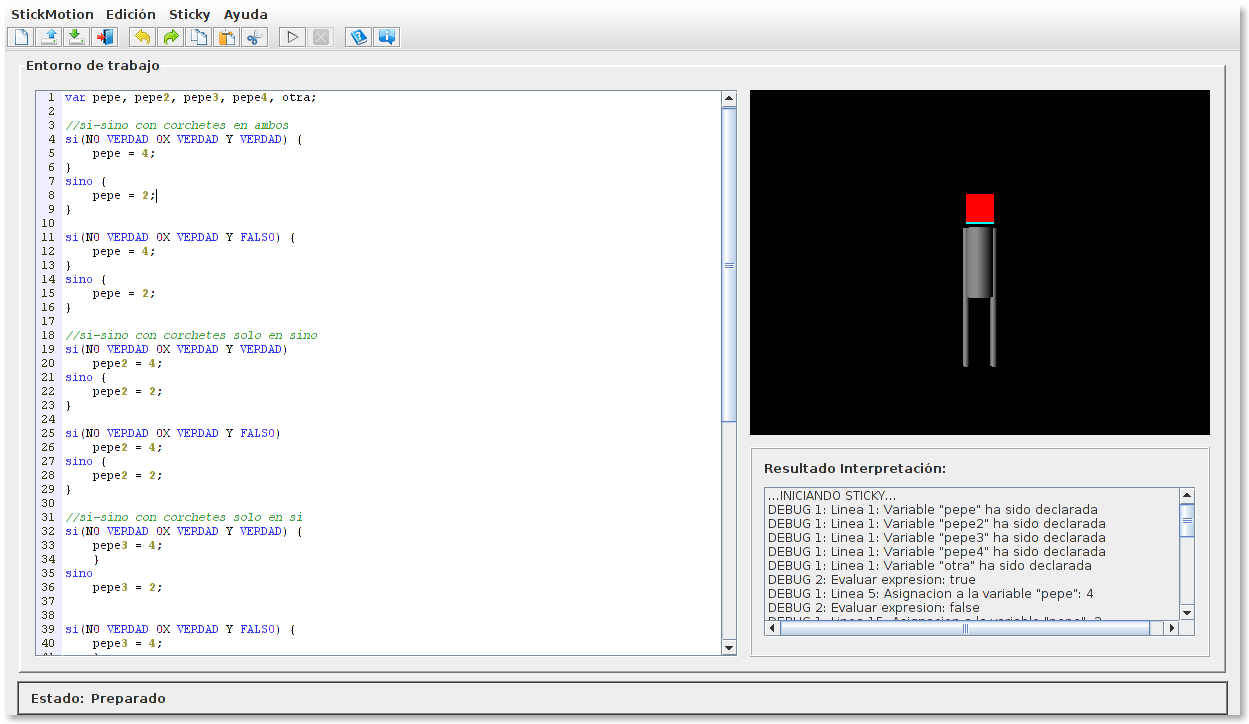
\includegraphics[width=\textwidth]{./imagenes/if.png}}
    \caption{Ejecución del ejemplo IF}
  \end{figure}
  

  \begin{figure}[htb]
    \centerline{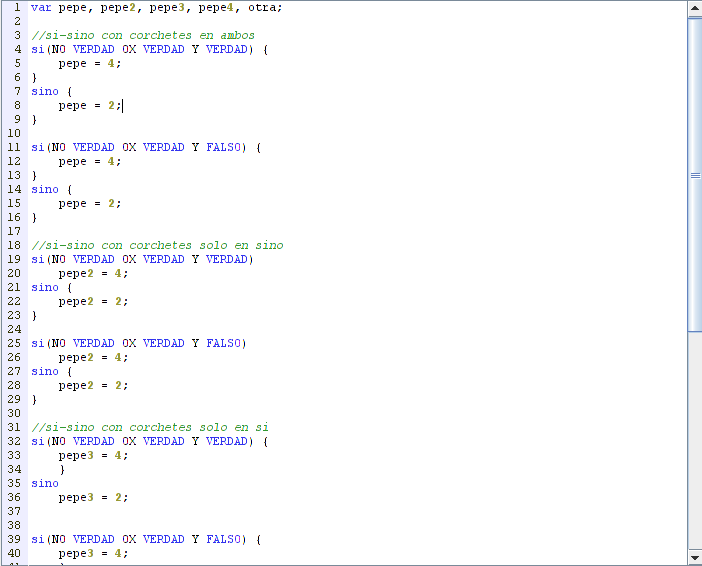
\includegraphics[width=\textwidth]{./imagenes/if-codigo.png}}
    \caption{Código del ejemplo IF Código}
  \end{figure}
  
  
  \begin{figure}[htb]
\centerline{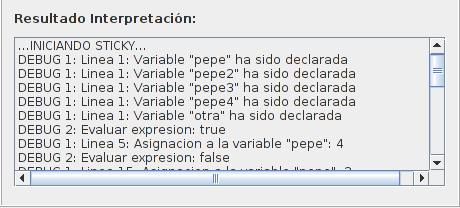
\includegraphics[width=\textwidth]{./imagenes/if-resultado.png}}
\caption{Resultado del ejemplo IF}
\end{figure}



\item Prueba de "mientras"\\
  
  

\begin{verbatim}
//Con corchetes
var otra = 0;
var contador=1;
mientras(contador < 10){
    otra++;
    mostrar("Valor de otra: "+otra);
    contador++;
}

//Sin corchetes
contador=1;
mientras(contador < 10)
    contador++;

$
\end{verbatim}

  
  
  \begin{itemize}
  \item Salida (Nivel de Debug 2 $\rightarrow$ Información auxiliar)
  \end{itemize}
\begin{verbatim}
...INICIANDO STICKY...
DEBUG 1: Linea 2: Variable "otra" ha sido declarada con valor 0
DEBUG 1: Linea 3: Variable "contador" ha sido declarada con valor 1
DEBUG 2: Evaluar expresion: true
Valor de otra: 1
DEBUG 2: Evaluar expresion: true
Valor de otra: 2
DEBUG 2: Evaluar expresion: true
Valor de otra: 3
DEBUG 2: Evaluar expresion: true
Valor de otra: 4
DEBUG 2: Evaluar expresion: true
Valor de otra: 5
DEBUG 2: Evaluar expresion: true
Valor de otra: 6
DEBUG 2: Evaluar expresion: true
Valor de otra: 7
DEBUG 2: Evaluar expresion: true
Valor de otra: 8
DEBUG 2: Evaluar expresion: true
Valor de otra: 9
DEBUG 2: Evaluar expresion: false
DEBUG 1: Linea 11: Asignacion a la variable "contador": 1
DEBUG 2: Evaluar expresion: true
DEBUG 2: Evaluar expresion: true
DEBUG 2: Evaluar expresion: true
DEBUG 2: Evaluar expresion: true
DEBUG 2: Evaluar expresion: true
DEBUG 2: Evaluar expresion: true
DEBUG 2: Evaluar expresion: true
DEBUG 2: Evaluar expresion: true
DEBUG 2: Evaluar expresion: true
DEBUG 2: Evaluar expresion: false
...FINALIZANDO STICKY...
\end{verbatim}

  
  
  
\item Bucle "para"\\
  
  
  
\begin{verbatim}
//Sin corchetes
var bucle = 1;
para(bucle;bucle < 10;2) 
    mostrar("Este es el valor de bucle: "+bucle);

//Con corchetes
bucle = 1;
para(bucle;bucle < 10;2)  {
    mostrar("Este es el valor de bucle: "+bucle);
    }
$
\end{verbatim}
  
  
  
  \begin{itemize}
  \item Salida (Nivel de Debug 2 $\rightarrow$ Información auxiliar)
  \end{itemize}
\begin{verbatim}
...INICIANDO STICKY...
DEBUG 1: Linea 2: Variable "bucle" ha sido declarada con valor 1
DEBUG 2: Evaluar expresion: true
Este es el valor de bucle: 3
DEBUG 2: Evaluar expresion: true
Este es el valor de bucle: 5
DEBUG 2: Evaluar expresion: true
Este es el valor de bucle: 7
DEBUG 2: Evaluar expresion: true
Este es el valor de bucle: 9
DEBUG 2: Evaluar expresion: true
Este es el valor de bucle: 11
DEBUG 2: Evaluar expresion: false
DEBUG 1: Linea 7: Asignacion a la variable "bucle": 1
DEBUG 2: Evaluar expresion: true
Este es el valor de bucle: 3
DEBUG 2: Evaluar expresion: true
Este es el valor de bucle: 5
DEBUG 2: Evaluar expresion: true
Este es el valor de bucle: 7
DEBUG 2: Evaluar expresion: true
Este es el valor de bucle: 9
DEBUG 2: Evaluar expresion: true
Este es el valor de bucle: 11
DEBUG 2: Evaluar expresion: false
...FINALIZANDO STICKY...
\end{verbatim}
  
  
  
  
\item Bloque "opcion"\\
  

  
\begin{verbatim}
var pepe = 3;

opcion (pepe) {
    caso 2: {
        mostrar("Caso 2");
        }fincaso;
    caso 3: {
        mostrar("Caso 3");
        }fincaso;
    caso VERDAD: {
        mostrar("Caso 4");
        }fincaso;
    
    caso "HOLA": {
        mostrar("Caso 5");
        }fincaso;
    
    defecto: {
        mostrar("pepito");
        } fincaso;
    
    }

pepe = "ninguna de esas";

opcion (pepe) {
    caso 2: {
        mostrar("Caso 2");
        }fincaso;
    caso 3: {
        mostrar("Caso 3");
        }fincaso;
    caso VERDAD: {
        mostrar("Caso 4");
        }fincaso;
    
    caso "HOLA": {
        mostrar("Caso 5");
        }fincaso;
    
    defecto: {
        mostrar("pepito");
        } fincaso;
    
    }
$
\end{verbatim}
  
  
  
  \begin{itemize}
\item Salida (Nivel de Debug 1 $\rightarrow$ Información básica)
\end{itemize}
\begin{verbatim}
...INICIANDO STICKY...
DEBUG 1: Linea 1: Variable "pepe" ha sido declarada con valor 3
Caso 3
DEBUG 1: Linea 24: Asignacion a la variable "pepe": "ninguna de esas"
pepito
...FINALIZANDO STICKY...
\end{verbatim}




\begin{figure}[htb]
  \centerline{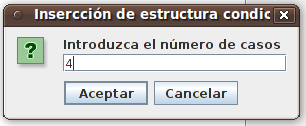
\includegraphics[width=\textwidth]{./imagenes/opcion.png}}
\caption{Ejecución del ejemplo Opcion}
\end{figure}


\begin{figure}[htb]
  \centerline{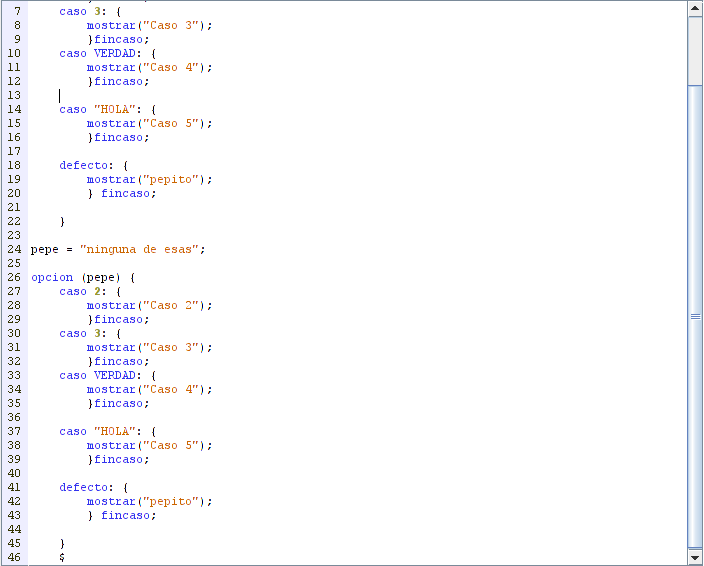
\includegraphics[width=\textwidth]{./imagenes/opcion-codigo.png}}
  \caption{Código del ejemplo Opcion}
\end{figure}


\begin{figure}[htb]
  \centerline{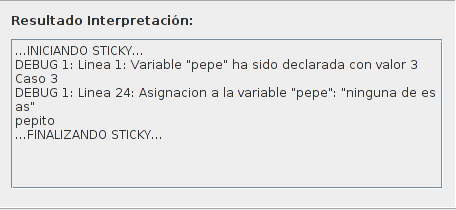
\includegraphics[width=\textwidth]{./imagenes/opcion-resultado.png}}
  \caption{Resultado del ejemplo Opcion}
\end{figure}



\end{itemize} % ends low level
\subsection{Ejemplos de Sticky}

\begin{itemize}
  
\item ¡Hola!\\
  

  
\begin{verbatim}
/*
    Ejemplo para decir hola
*/

girar BRAZO DER (1, 2.3, 1500);
girar BRAZO DER (2.60, 0, 500);

tiempo avanza (1500);
var contador = 0;
var neg = (-3.14/2.5);
var pos = -neg;
mientras(contador < 10) {
tiempo avanza (350);

si (contador%2 == 0)
    flexionar BRAZO DER (neg, 200);
sino 
    flexionar BRAZO DER (pos, 200);
    
contador++;
}

$
\end{verbatim}
  

  
  \begin{itemize}
  \item Salida (Nivel de Debug 0 $\rightarrow$ Errores)
  \end{itemize}
\begin{verbatim}
...INICIANDO STICKY...
...FINALIZANDO STICKY...
\end{verbatim}
  
  
  
  \begin{figure}[htb]
    \centerline{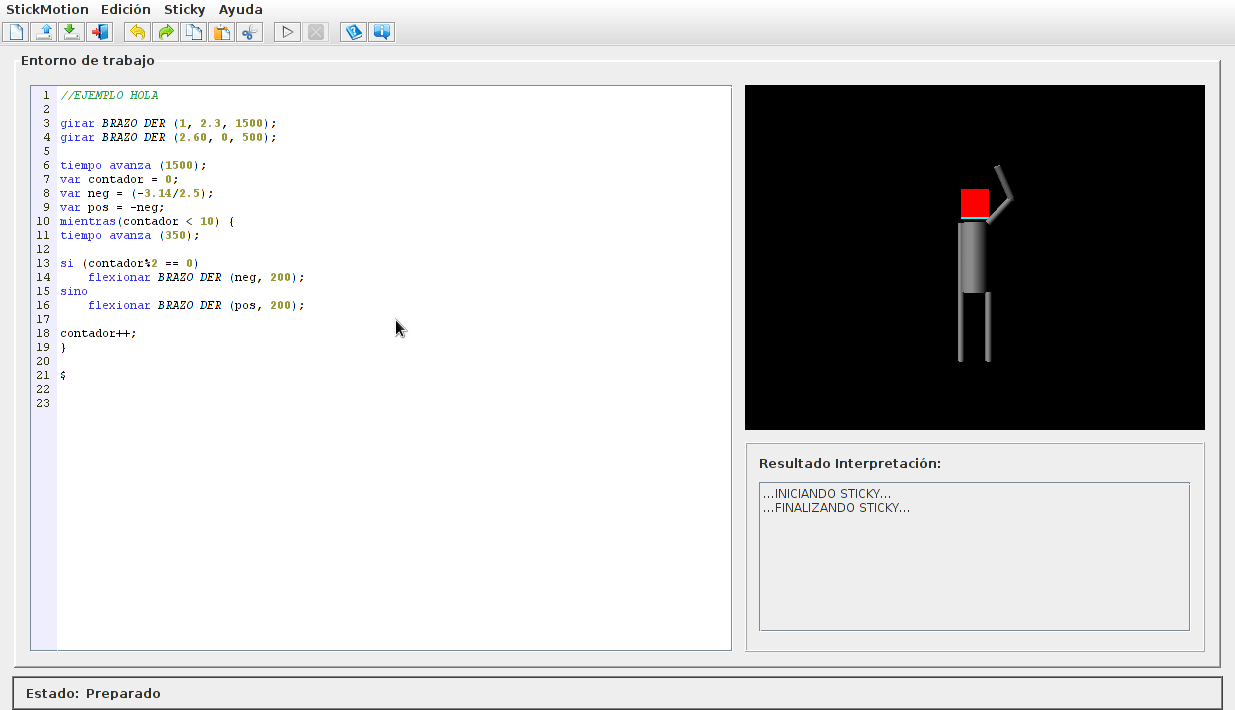
\includegraphics[width=\textwidth]{./imagenes/hola.png}}
    \caption{Ejecución del ejemplo Hola}
  \end{figure}
  
  
\begin{figure}[htb]
  \centerline{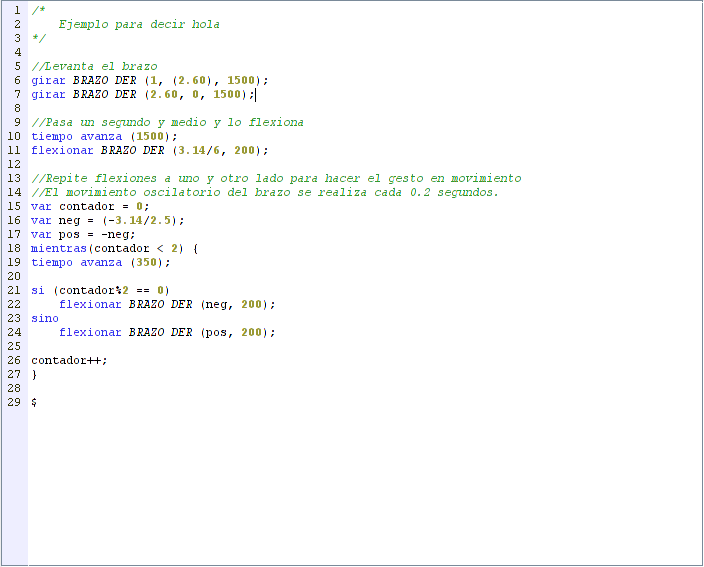
\includegraphics[width=\textwidth]{./imagenes/hola-codigo.png}}
  \caption{Código del ejemplo Hola}
\end{figure}


\begin{figure}[htb]
  \centerline{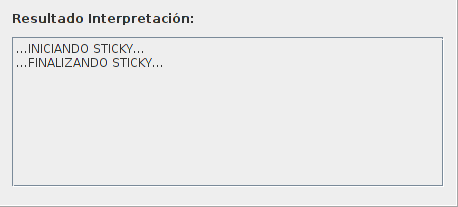
\includegraphics[width=\textwidth]{./imagenes/hola-resultado.png}}
\caption{Resultado del ejemplo Hola}
\end{figure}


\begin{figure}[htb]
  \centerline{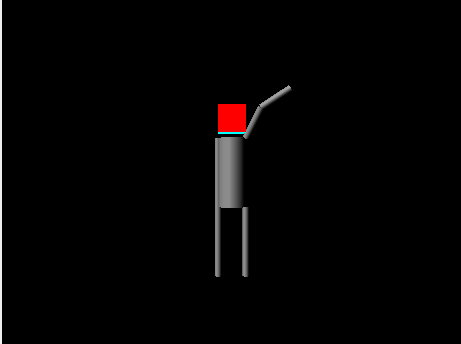
\includegraphics[width=\textwidth]{./imagenes/hola-stickman.png}}
  \caption{Stickman del ejemplo Hola}
\end{figure}



\item Andar\\
  
  
  
\begin{verbatim}
/*
    Stickman caminando de forma realista
*/
//Posiciona a Steve a la izquierda de la pantalla mirando hacia la derecha.
mover STICKMAN (-2,0,0,200);
girar STICKMAN (PI/2,0,200);
tiempo avanza (200);

//Variables para andar
var t=500;
var angulo=PI/8;
var iteraciones=2;
var i=0;


//Andar hacia la derecha---------------------------------------------------
para(i; i<iteraciones; 1) {

    //Primer pasito------------------------------------------
    girar STICKMAN (0,0.05,t);
    
    //Encoge la pierna izquierda
    girar PIERNA IZQ (0,angulo,t);
    flexionar PIERNA IZQ (angulo,t);
    mover STICKMAN (0,0.5,0.05,t);

    //Avanza la pierna derecha
    flexionar PIERNA DER (angulo,t);
    girar PIERNA DER (0,-angulo*2,t);

    //Inclina a Steve hacia adelante
    girar STICKMAN (0,-0.1,t);

    //Mueve los brazos
    girar BRAZO DER (0,0.1,t);
    girar BRAZO IZQ (0,-0.1,t);


    tiempo avanza (t);

    //Apoya la pierna derecha
    mover STICKMAN (0,0.5,-0.05,t);
    flexionar PIERNA DER (-angulo,t);
    girar PIERNA DER (0,angulo*2,t);

    //Estira la pierna izquierda
    girar PIERNA IZQ (0,-angulo,t);
    flexionar PIERNA IZQ (-angulo,t);

    //Inclina a Steve hacia su posicion inicial
    girar STICKMAN (0,0.05,t);

    
    //Mueve los brazos
    girar BRAZO DER (0,-0.1,t);
    girar BRAZO IZQ (0,0.1,t);
    
    tiempo avanza(t);
    //-------------------------------------------------------

    //Segundo pasito-----------------------------------------
    girar STICKMAN (0,0.05,t);
    
    //Encoge la pierna izquierda
    girar PIERNA DER (0,angulo,t);
    flexionar PIERNA DER (angulo,t);
    mover STICKMAN (0,0.5,0.05,t);

    //Avanza la pierna derecha
    flexionar PIERNA IZQ (angulo,t);
    girar PIERNA IZQ (0,-angulo*2,t);

    //Inclina a Steve hacia adelante
    girar STICKMAN (0,-0.1,t);

    //Mueve los brazos
    girar BRAZO DER (0,-0.1,t);
    girar BRAZO IZQ (0,0.1,t);

    tiempo avanza (t);


    //Apoya la pierna derecha
    mover STICKMAN (0,0.5,-0.05,t);
    flexionar PIERNA IZQ (-angulo,t);
    girar PIERNA IZQ (0,angulo*2,t);

    //Estira la pierna izquierda
    girar PIERNA DER (0,-angulo,t);
    flexionar PIERNA DER (-angulo,t);

    //Inclina a Steve hacia su posicion inicial
    girar STICKMAN (0,0.05,t);
    
    //Mueve los brazos
    girar BRAZO DER (0,0.1,t);
    girar BRAZO IZQ (0,-0.1,t);

    tiempo avanza(t);
    //-------------------------------------------------------

}
//-------------------------------------------------------------------------


//Se mueve hacia la izquierda----------------------------------------------
girar STICKMAN (PI,0,200);
tiempo avanza (200);
i=0;

para(i; i<iteraciones; 1) {

    //Primer pasito------------------------------------------
    girar STICKMAN (0,0.05,t);
    
    //Encoge la pierna izquierda
    girar PIERNA IZQ (0,angulo,t);
    flexionar PIERNA IZQ (angulo,t);
    mover STICKMAN (0,0.5,0.05,t);

    //Avanza la pierna derecha
    flexionar PIERNA DER (angulo,t);
    girar PIERNA DER (0,-angulo*2,t);

    //Inclina a Steve hacia adelante
    girar STICKMAN (0,-0.1,t);

    //Mueve los brazos
    girar BRAZO DER (0,0.1,t);
    girar BRAZO IZQ (0,-0.1,t);


    tiempo avanza (t);

    //Apoya la pierna derecha
    mover STICKMAN (0,0.5,-0.05,t);
    flexionar PIERNA DER (-angulo,t);
    girar PIERNA DER (0,angulo*2,t);

    //Estira la pierna izquierda
    girar PIERNA IZQ (0,-angulo,t);
    flexionar PIERNA IZQ (-angulo,t);

    //Inclina a Steve hacia su posicion inicial
    girar STICKMAN (0,0.05,t);

    
    //Mueve los brazos
    girar BRAZO DER (0,-0.1,t);
    girar BRAZO IZQ (0,0.1,t);
    
    tiempo avanza(t);
    //-------------------------------------------------------

    //Segundo pasito-----------------------------------------
    girar STICKMAN (0,0.05,t);
    
    //Encoge la pierna izquierda
    girar PIERNA DER (0,angulo,t);
    flexionar PIERNA DER (angulo,t);
    mover STICKMAN (0,0.5,0.05,t);

    //Avanza la pierna derecha
    flexionar PIERNA IZQ (angulo,t);
    girar PIERNA IZQ (0,-angulo*2,t);

    //Inclina a Steve hacia adelante
    girar STICKMAN (0,-0.1,t);

    //Mueve los brazos
    girar BRAZO DER (0,-0.1,t);
    girar BRAZO IZQ (0,0.1,t);

    tiempo avanza (t);


    //Apoya la pierna derecha
    mover STICKMAN (0,0.5,-0.05,t);
    flexionar PIERNA IZQ (-angulo,t);
    girar PIERNA IZQ (0,angulo*2,t);

    //Estira la pierna izquierda
    girar PIERNA DER (0,-angulo,t);
    flexionar PIERNA DER (-angulo,t);

    //Inclina a Steve hacia su posicion inicial
    girar STICKMAN (0,0.05,t);
    
    //Mueve los brazos
    girar BRAZO DER (0,0.1,t);
    girar BRAZO IZQ (0,-0.1,t);

    tiempo avanza(t);
    //-------------------------------------------------------

}
//-------------------------------------------------------------------------

$
\end{verbatim}
  
  
  
  
\begin{figure}[htb]
  \centerline{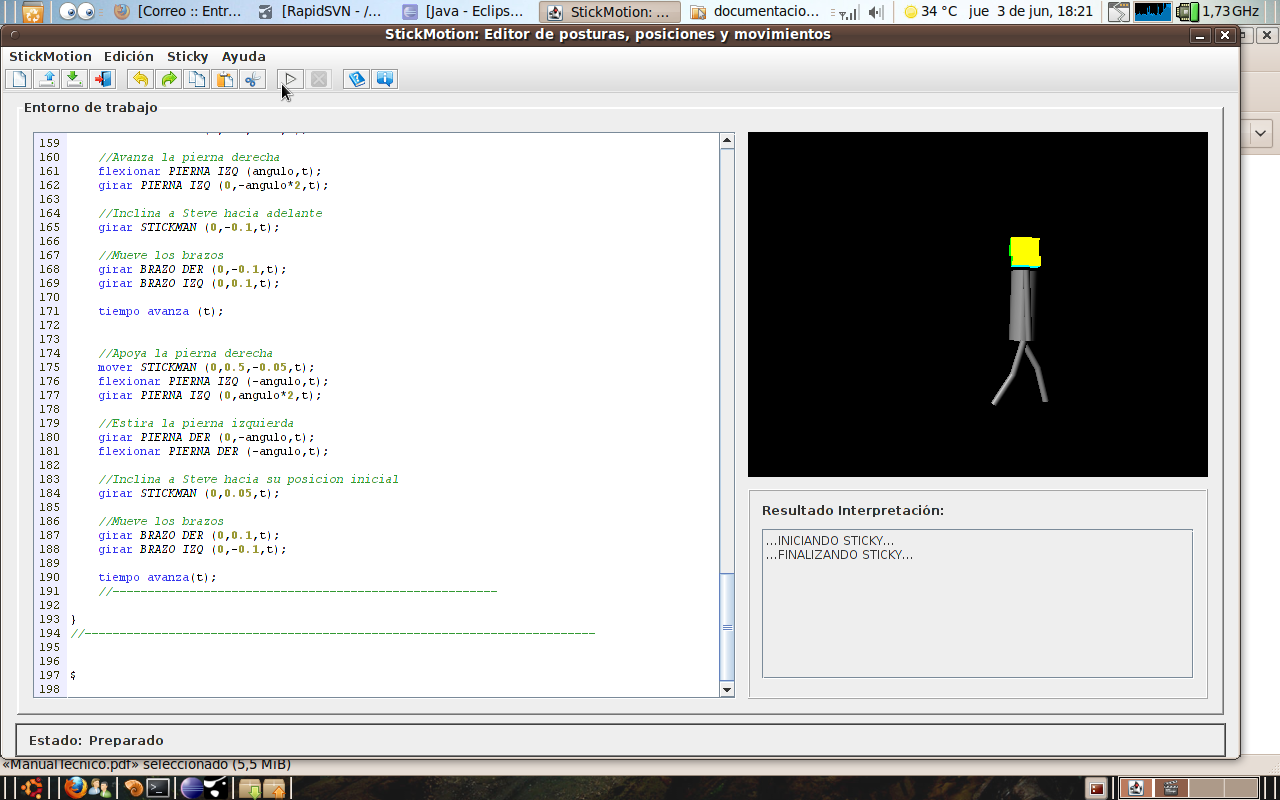
\includegraphics[width=\textwidth]{./imagenes/andar.png}}
  \caption{Ejecución del ejemplo Andar}
\end{figure}


\begin{figure}[htb]
  \centerline{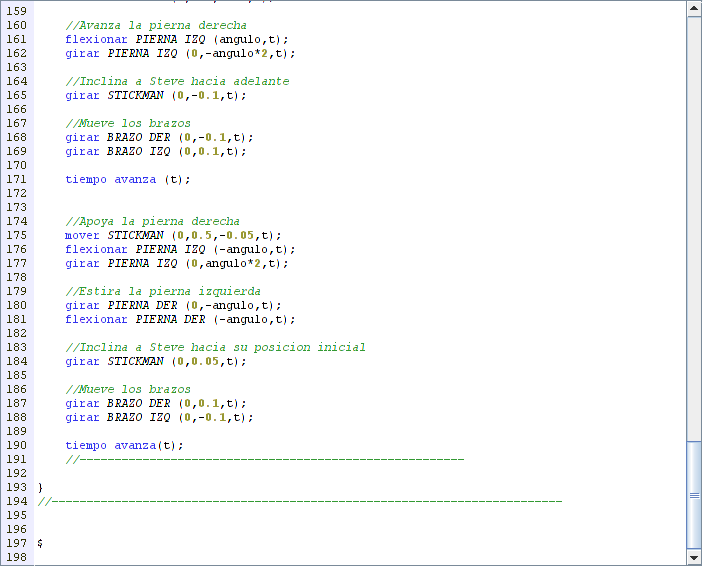
\includegraphics[width=\textwidth]{./imagenes/andar-codigo.png}}
\caption{Código del ejemplo Andar}
\end{figure}


\begin{figure}[htb]
  \centerline{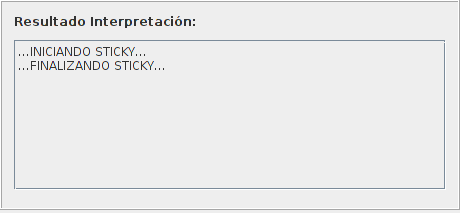
\includegraphics[width=\textwidth]{./imagenes/andar-resultado.png}}
  \caption{Resultado del ejemplo Andar}
\end{figure}


\begin{figure}[htb]
  \centerline{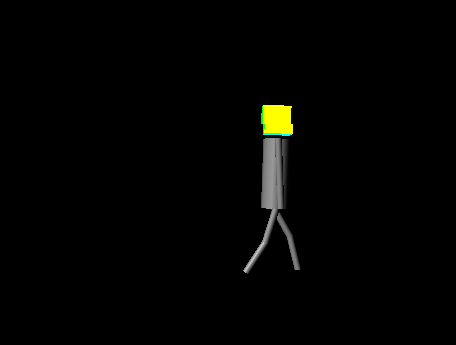
\includegraphics[width=\textwidth]{./imagenes/andar-stickman.png}}
  \caption{Stickman del ejemplo Andar}
\end{figure}



\item Haciendo el pino\\



\begin{verbatim}
/*
    Stickman haciendo el pino
*/

girar STICKMAN (3.14/2 , 0 , 1000);
tiempo avanza (1000);
girar BRAZO IZQ (0 , (-3.1) ,1000);
girar BRAZO DER (0 , 3.1 , 1000);
girar STICKMAN (0, (-3.14) ,1000);
flexionar PIERNA IZQ ( 3.14/8, 500);
flexionar PIERNA DER (3.14/8 , 500 );
girar PIERNA IZQ (0, 3.14/8 , 1000);
girar PIERNA DER (0 , (-3.14/8) , 1000);
flexionar PIERNA IZQ ( 3.14/8,  500);
flexionar PIERNA DER ( -3.14/8 , 500 );
tiempo avanza (1000);
flexionar BRAZO IZQ ( (-3.14/8) , 500);
flexionar BRAZO DER ( (-3.14/8) , 500 );
tiempo avanza (2000);

flexionar BRAZO IZQ ( (-3.14/8) , 500);
flexionar BRAZO DER (3.14/8 , 500);
girar BRAZO IZQ (0, 3.1, 1500);

flexionar PIERNA IZQ ((-3.14/4), 500);
flexionar PIERNA DER ((3.14/4), 500);
girar PIERNA IZQ (0, (-3.14/8), 1000);
girar PIERNA DER (0, (3.14/8), 1000);
tiempo avanza (50);
girar STICKMAN ((-3.14/2), 0, 1000);


//vuelve a su posicion
tiempo avanza (2000);
girar STICKMAN (3.14 , 3.14, 1000);
girar BRAZO DER (0, (-3.1), 1500);
flexionar PIERNA DER ((-3.14/4), 500);
flexionar BRAZO IZQ ((3.14/4), 500);

$
\end{verbatim}



\begin{figure}[htb]
  \centerline{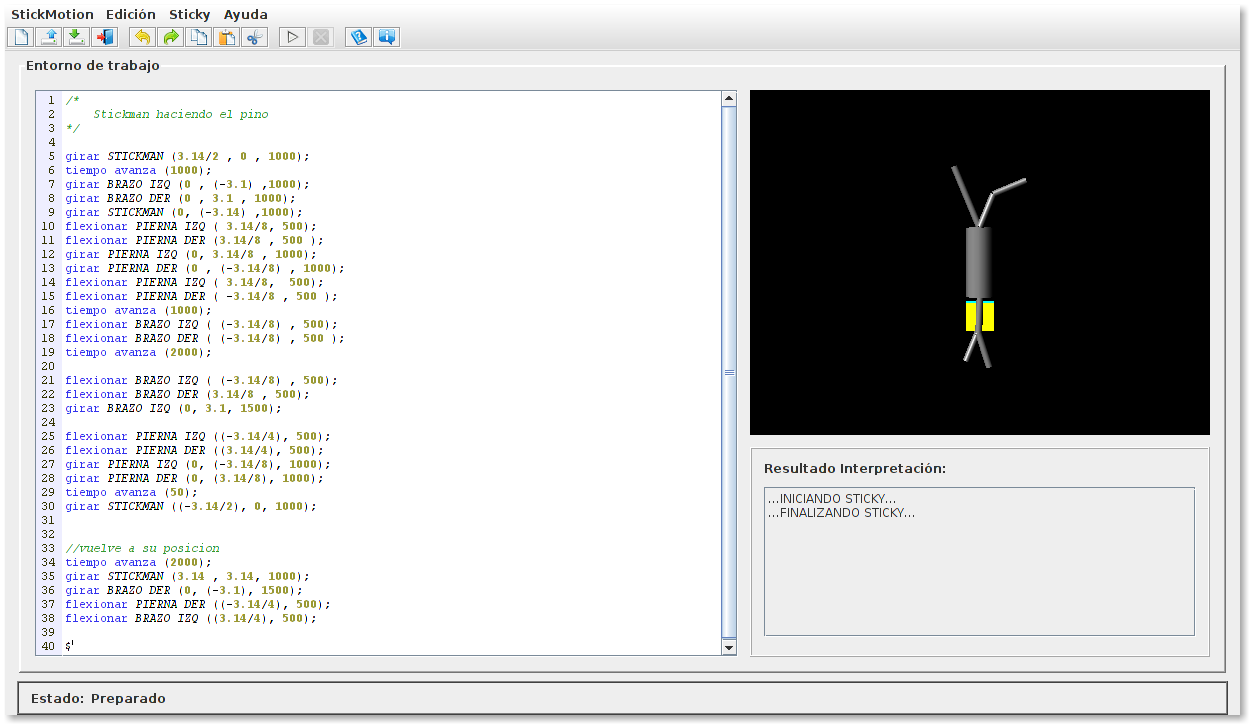
\includegraphics[width=\textwidth]{./imagenes/pino1.png}}
  \caption{Ejecución del ejemplo Pino}
\end{figure}

\begin{figure}[htb]
  \centerline{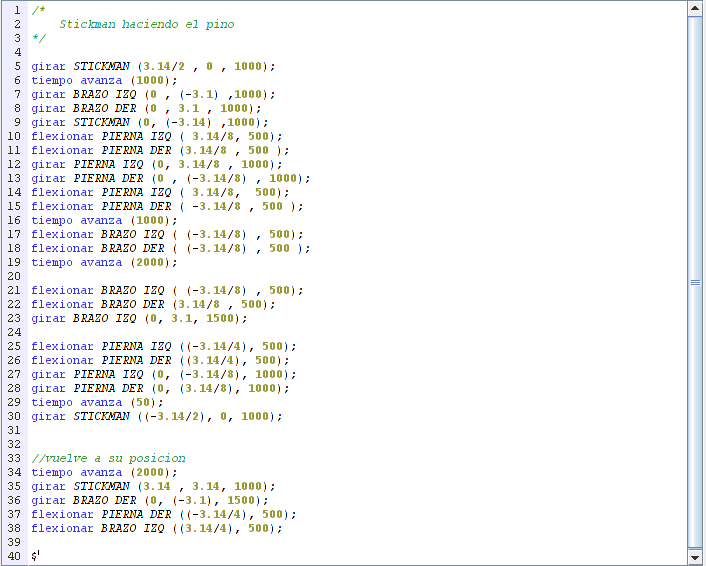
\includegraphics[width=\textwidth]{./imagenes/pino1-codigo.png}}
  \caption{Código del ejemplo Pino}
\end{figure}


\begin{figure}[htb]
  \centerline{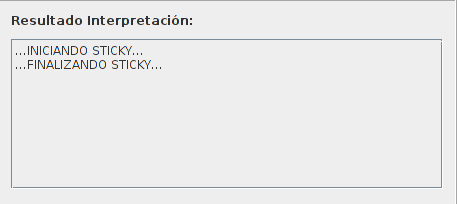
\includegraphics[width=\textwidth]{./imagenes/pino1-resultado.png}}
  \caption{Resultado del ejemplo Pino}
\end{figure}

\begin{figure}[htb]
  \centerline{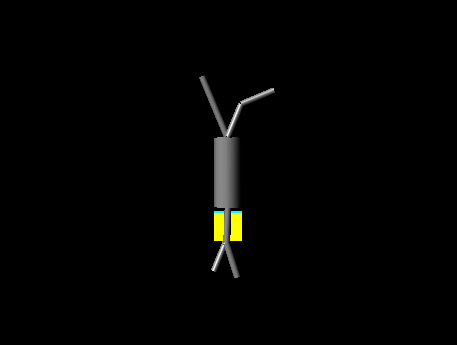
\includegraphics[width=\textwidth]{./imagenes/pino1-stickman.png}}
  \caption{Stickman del ejemplo Pino}
\end{figure}

\begin{figure}[htb]
  \centerline{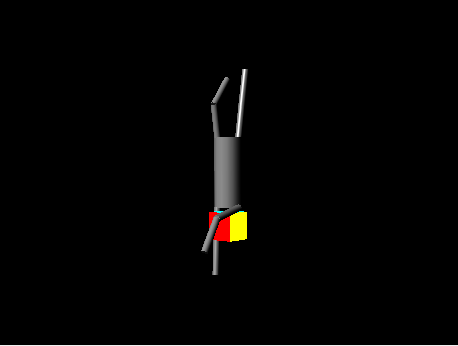
\includegraphics[width=\textwidth]{./imagenes/pino2-stickman.png}}
  \caption{Stickman del ejemplo Pino}
\end{figure}

\begin{figure}[htb]
  \centerline{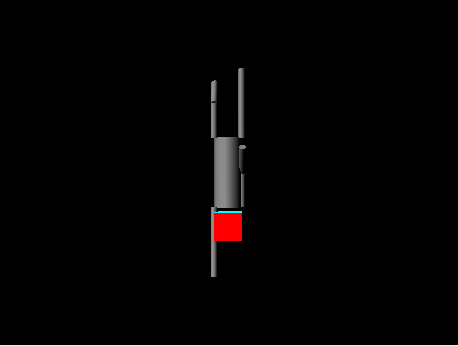
\includegraphics[width=\textwidth]{./imagenes/pino3-stickman.png}}
  \caption{Stickman del ejemplo Pino}
\end{figure}


\item Sticky Michael Jackson "Moonwalk"\\
  

  
\begin{verbatim}
/* 
    Michael Jackson "Moonwalk"
    Tipico baile con pasos hacia atras del mitico Rey del Pop.
    El giro es en espiral.
*/

//Stickman va girando hacia atras en espiral
girar STICKMAN (PI*2, 0, 8000);
mover STICKMAN (2, 0, 0, 8000);

//Realizando 4 pasos Moonwalk completos con cada pierna hacia atras
var contador = 4;
mientras(contador!=0) {
    
    flexionar PIERNA IZQ (PI/6, 700);
    girar PIERNA IZQ (0, -PI/4, 700);
    
    tiempo avanza (700);
    flexionar PIERNA IZQ ((-PI/6), 700);
    girar PIERNA IZQ (0, (PI/4), 700);
    flexionar PIERNA DER (PI/6, 700);
    girar PIERNA DER (0, (-PI/4), 700);


    tiempo avanza (700);
    flexionar PIERNA DER (-PI/6, 700);
    girar PIERNA DER (0, (PI/4), 700);
       tiempo avanza (700);
    contador--;
    }

$
\end{verbatim}
  
  
  
  \begin{figure}[htb]
    \centerline{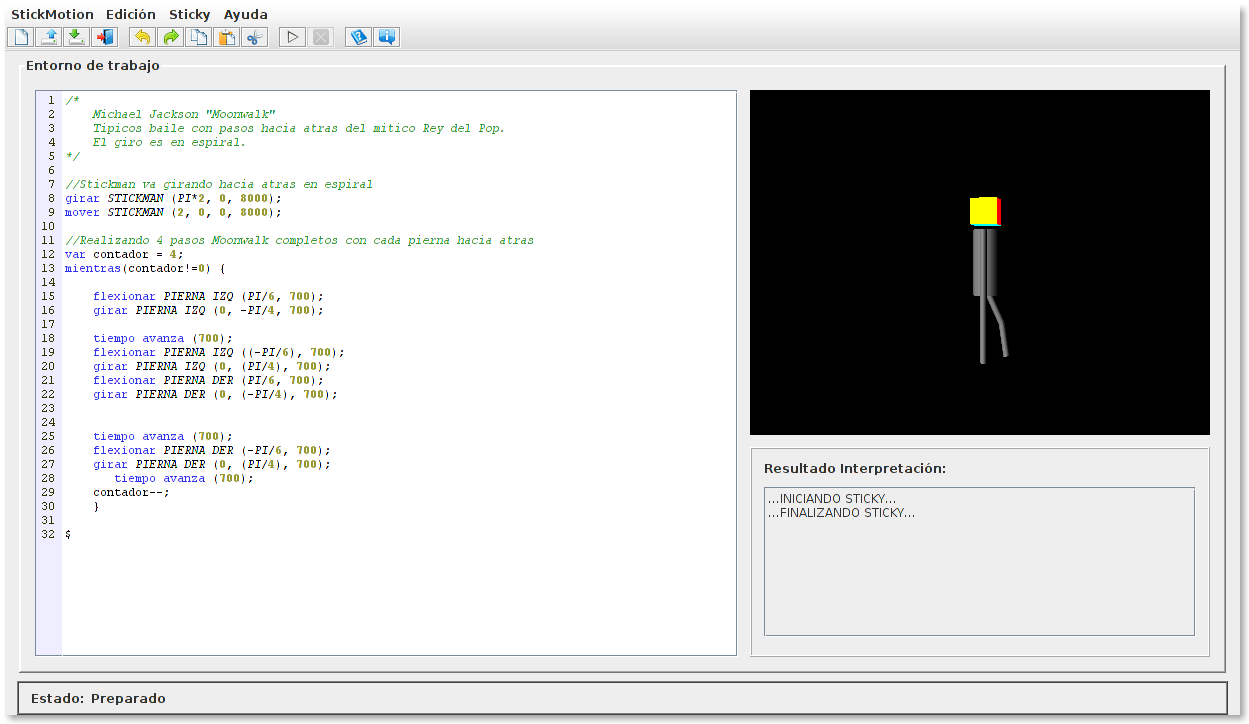
\includegraphics[width=\textwidth]{./imagenes/moonwalk.png}}
    \caption{Ejecución del ejemplo Moonwalk}
  \end{figure}
  

  \begin{figure}[htb]
    \centerline{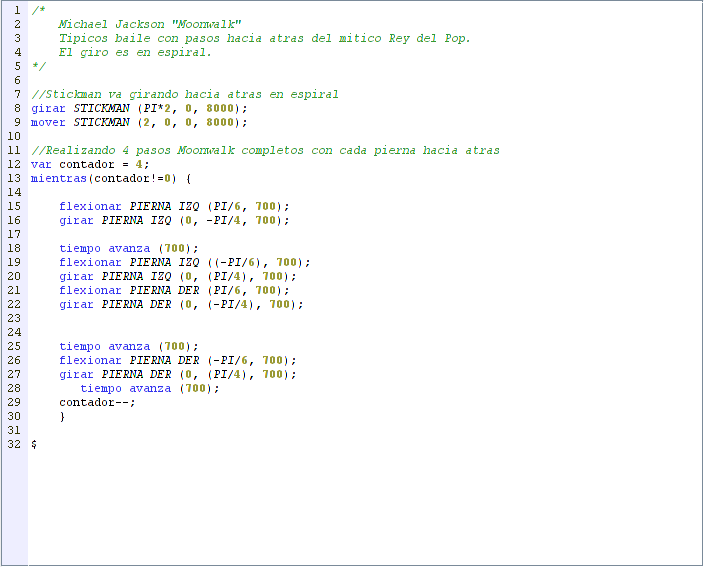
\includegraphics[width=\textwidth]{./imagenes/moonwalk-codigo.png}}
    \caption{Ejecución del ejemplo Moonwalk}
  \end{figure}
  
  
  
\begin{figure}[htb]
  \centerline{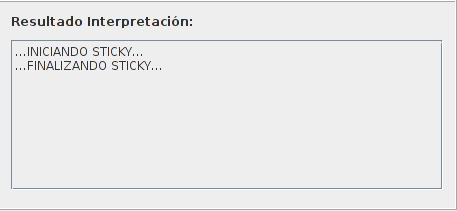
\includegraphics[width=\textwidth]{./imagenes/moonwalk-resultado.png}}
  \caption{Resultado del ejemplo Moonwalk}
\end{figure}


\begin{figure}[htb]
  \centerline{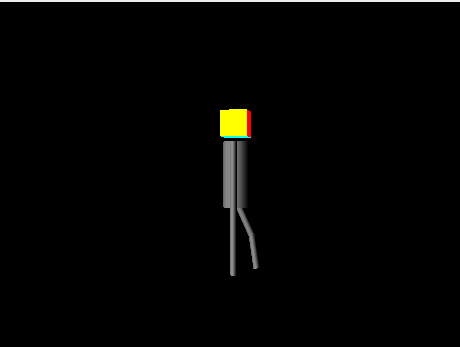
\includegraphics[width=\textwidth]{./imagenes/moonwalk-stickman.png}}
  \caption{Stickman del ejemplo Moonwalk}
\end{figure}


\begin{figure}[htb]
  \centerline{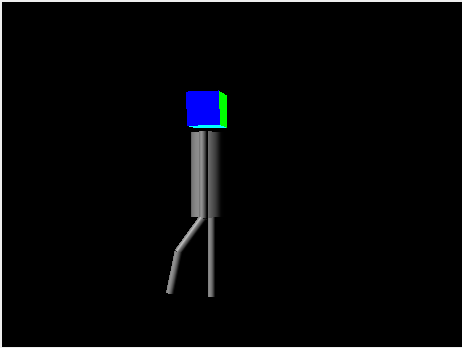
\includegraphics[width=\textwidth]{./imagenes/moonwalk2-stickman.png}}
  \caption{Stickman del ejemplo Moonwalk}
\end{figure}





\item Volando\\
  
  
  
\begin{verbatim}
////////////////
var d= 300; // duration for the movements

// Rotate the arms to move sideways
girar BRAZO DER (PI/2, 0, 50);
girar BRAZO IZQ (PI/2, 0, 50);

// walk
var i=0;
para(i; i < 20; 1) {  
  girar PIERNA DER(0,PI/2,d);
  girar PIERNA IZQ(0,-PI/2,d);
  flexionar PIERNA DER(PI/3,d);
  flexionar PIERNA IZQ(PI/3,d);
  tiempo avanza (d);
  girar PIERNA DER(0,-PI/2,d);
  girar PIERNA IZQ(0,PI/2,d);
  flexionar PIERNA DER(-PI/3,d);
  flexionar PIERNA IZQ(-PI/3,d);
  tiempo avanza (d);  
}


// Try to fly
i=0;
tiempo establece(2000);
tiempo avanza (d);
para(i; i < 16; 1) {    
    girar BRAZO DER(0, PI / 2, d);
    girar BRAZO IZQ(0, PI / 2, d);
    // flex forearms
    flexionar BRAZO DER(PI / 4, d);
    flexionar BRAZO IZQ(PI / 4, d);
    // next step
    tiempo avanza (d);
    girar BRAZO DER(0, -PI / 2, d);
    girar BRAZO IZQ(0, -PI / 2, d);
    // un-Flex forearms
    flexionar BRAZO DER(-PI / 4, d);
    flexionar BRAZO IZQ(-PI / 4, d);
    tiempo avanza (d);
} 


// Fly up
tiempo establece (2500);
i=0;
para(i; i < 30; 1) {
  mover STICKMAN (0.1,-0.3,-0.15, d);
  tiempo avanza (d);
}
// Fall down
tiempo establece (2500 + 30*d);
girar STICKMAN (0,-PI/2,d/2);
tiempo avanza (d/2);
mover STICKMAN (0,9,0,d);

$
\end{verbatim}
  
  
  
  \begin{itemize}
\item Salida (Nivel de Debug 0 $\rightarrow$ Errores)
\end{itemize}
\begin{figure}[htb]
  \centerline{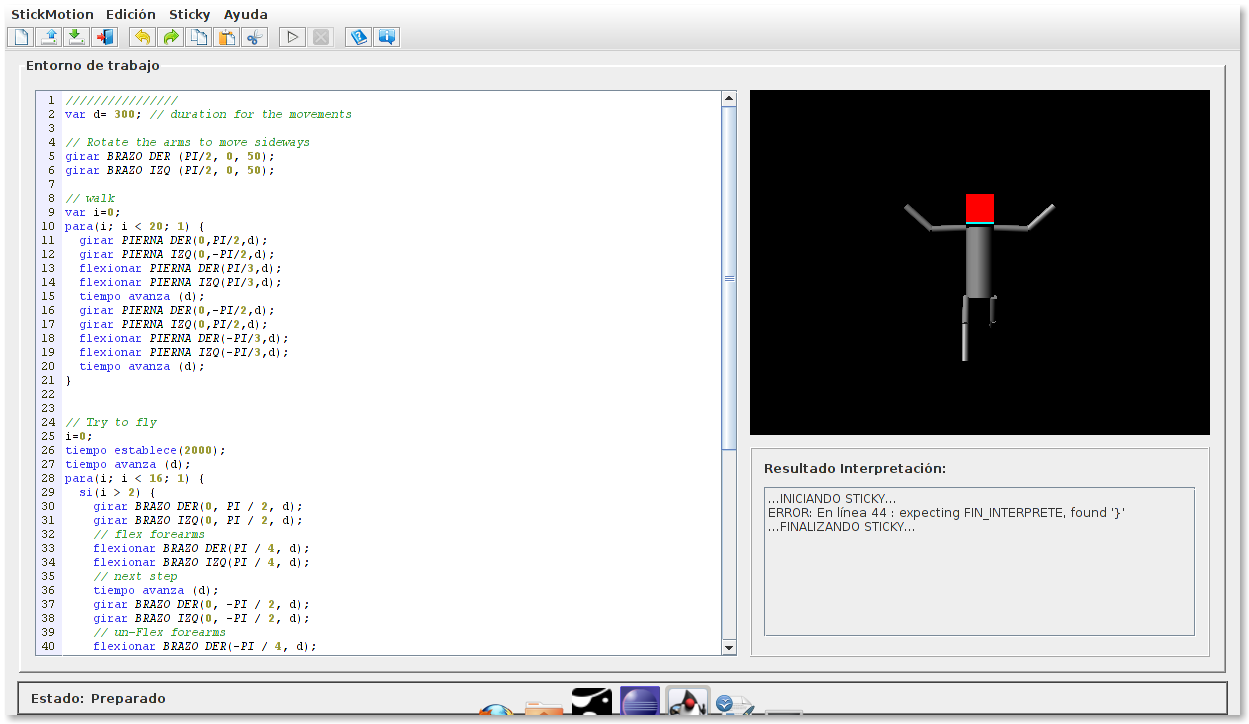
\includegraphics[width=\textwidth]{./imagenes/volar1.png}}
  \caption{Ejecución del ejemplo Volar}
\end{figure}


\begin{figure}[htb]
  \centerline{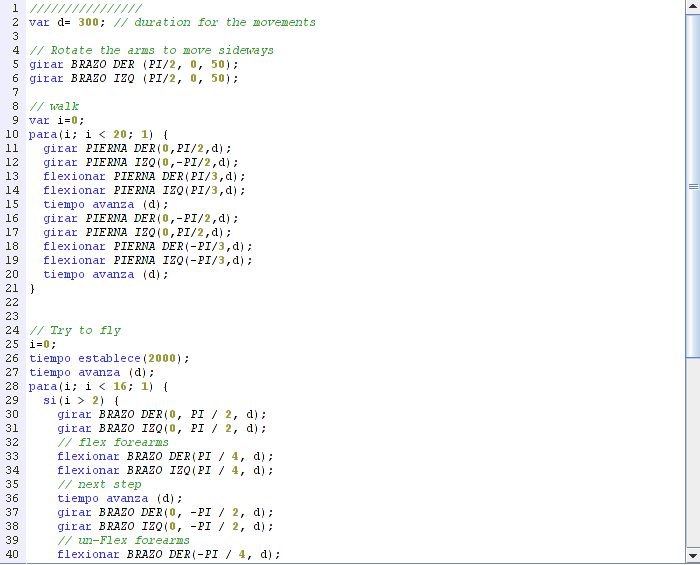
\includegraphics[width=\textwidth]{./imagenes/volar1-codigo.png}}
\caption{Código del ejemplo Volar}
\end{figure}


\begin{figure}[htb]
  \centerline{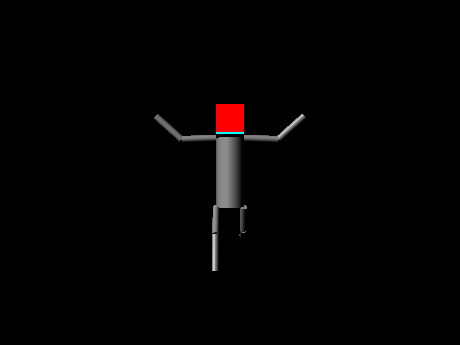
\includegraphics[width=\textwidth]{./imagenes/volar1-stickman.png}}
  \caption{Stickman del ejemplo Volar}
\end{figure}



\item Sticky Street Fighter\\
  
  
  
\begin{verbatim}
//--------------------------------------------- 
// STREET FIGHTER 
/* 
    Street Fighter Ryu 
    Shoryuken y patada giratoria ( a lo Chuck Norris ). 
*/ 

var t =  1000; 

girar STICKMAN (2, 0, t); 
tiempo avanza (t); 
mover STICKMAN (0, 1, 0, t/2); 
tiempo avanza (t/2); 
girar STICKMAN (2*PI, 0, t); 
mover STICKMAN (0,0.5,-1.5,t); 
girar BRAZO IZQ (0,-3,t); 
flexionar BRAZO DER (PI/2, t); 
flexionar BRAZO IZQ (-PI/5, t); 
flexionar PIERNA IZQ(PI/3,t); 
flexionar PIERNA DER(PI/2,t); 
mostrar ("SHORYUKEN !!"); 
tiempo avanza (t); 
mover STICKMAN (-1,0,1.5,t); 
girar BRAZO IZQ (0,3,t); 
flexionar BRAZO DER (-PI/2, t); 
flexionar BRAZO IZQ (PI/5, t); 
flexionar PIERNA IZQ(-PI/3,t); 
flexionar PIERNA DER(-PI/2,t); 
tiempo avanza (t); 
girar PIERNA DER (0, PI/2, t); 
mover STICKMAN (0, -3, 0, t); 
girar STICKMAN (4*PI, 0 , t); 
tiempo avanza (t); 
girar STICKMAN (PI*4, 0, t); 
mover STICKMAN (2, 0 , 0, t); 
tiempo avanza (t); 
girar STICKMAN (PI/2, 0, t); 
girar PIERNA DER (0, -PI/2, t); 
tiempo avanza (t); 
mover STICKMAN (0,-5,0, t); 
flexionar PIERNA DER(-PI/3,t); 
girar PIERNA IZQ (0, PI/2, t); 
girar BRAZO IZQ (0, PI/2, t); 
girar BRAZO DER (0, PI/2, t); 
flexionar BRAZO DER (PI/2, t); 
tiempo avanza (t); 
girar STICKMAN (-PI/3, 0, t/3); 
mover STICKMAN (1,0,0, t/3); 
tiempo avanza (t/3); 
girar STICKMAN (PI/3.5, 0, t/3); 
mover STICKMAN (0,1,0, t/3 ); 
tiempo avanza (t/3); 
mover STICKMAN (0,-2.5,0.5, t/3); 

$
\end{verbatim}
  
  
  
  
  \begin{figure}[htb]
    \centerline{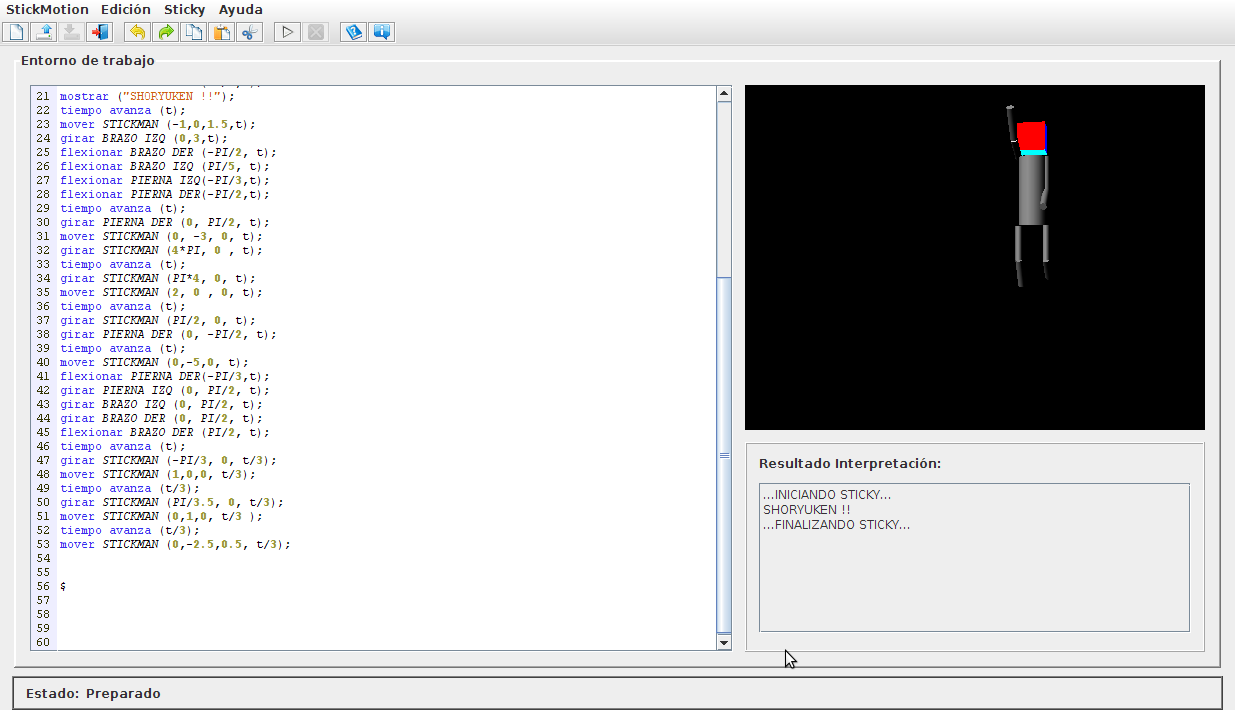
\includegraphics[width=\textwidth]{./imagenes/streetfighter1.png}}
    \caption{Ejecución del ejemplo Street Fighter}
\end{figure}

\begin{figure}[htb]
\centerline{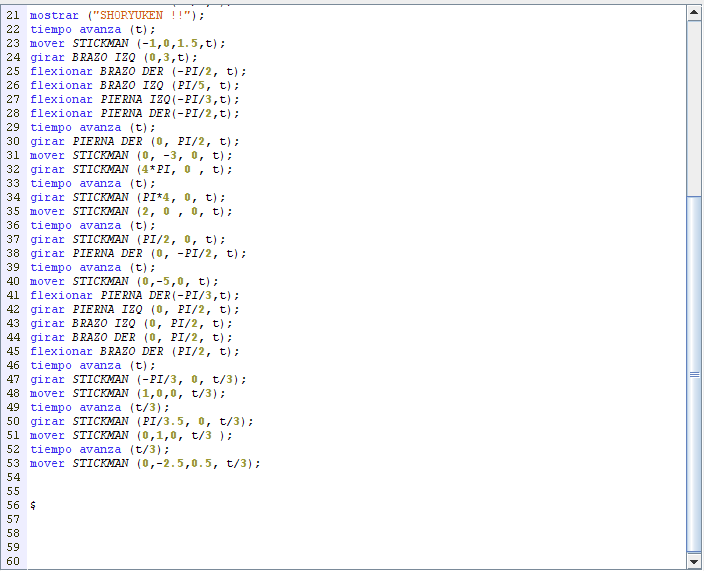
\includegraphics[width=\textwidth]{./imagenes/streetfighter-codigo.png}}
\caption{Código  del ejemplo Street Fighter}
\end{figure}


\begin{figure}[htb]
  \centerline{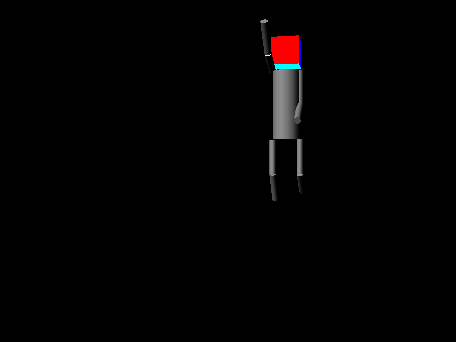
\includegraphics[width=\textwidth]{./imagenes/streetfighter-resultado1.png}}
  \caption{Animación del ejemplo Street Fighter}
\end{figure}

\begin{figure}[htb]
  \centerline{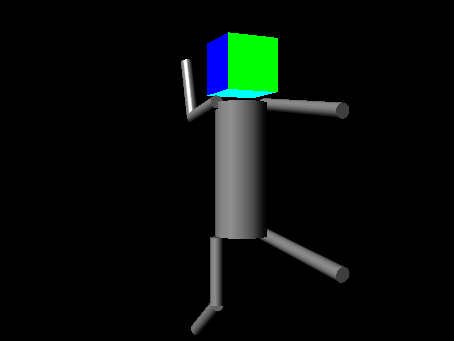
\includegraphics[width=\textwidth]{./imagenes/streetfighter-resultado2.png}}
  \caption{Animación del ejemplo Street Fighter}
\end{figure}


\item Corte de Mangas\\
  
  
  
\begin{verbatim}
//---------------------------------------------
// CORTE DE MANGAS
// Aprobaremos la asignatura: en este codigo esta la respuesta.

girar BRAZO DER (0, 3.14/5, 500);
flexionar BRAZO DER (3.14/1.8, 500);
girar BRAZO DER ((-3.14/2), 0, 700);
tiempo avanza (500);
girar BRAZO IZQ (0, (-3.14/6), 200);
flexionar BRAZO IZQ (-3.14/1.6, 300);


girar STICKMAN (3.14/2 , 0 , 1000);
    
$
\end{verbatim}

  
  
  \begin{figure}[htb]
    \centerline{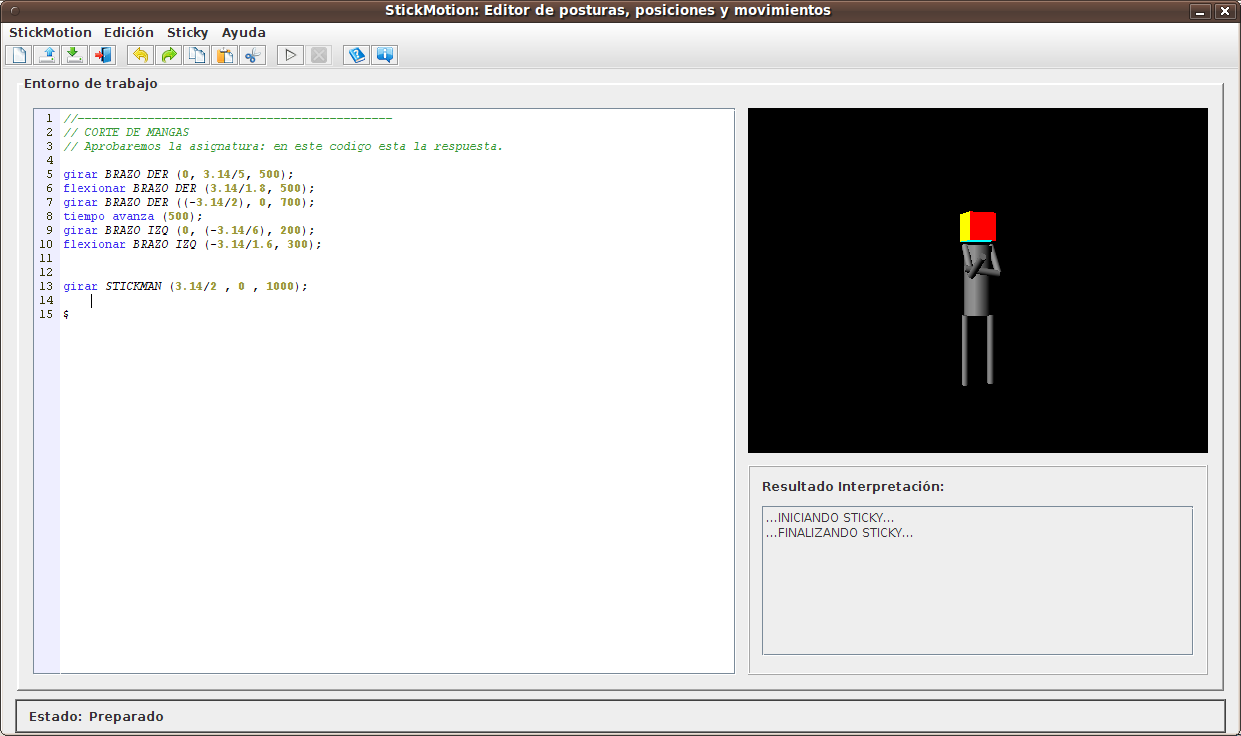
\includegraphics[width=\textwidth]{./imagenes/cortemangas.png}}
    \caption{Ejecución del ejemplo Corte de mangas}
  \end{figure}
  

  \begin{figure}[htb]
    \centerline{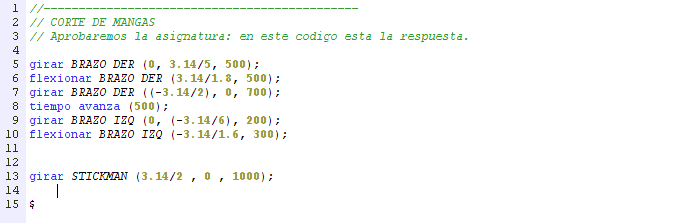
\includegraphics[width=\textwidth]{./imagenes/cortemangas-codigo.png}}
    \caption{Código del ejemplo Corte de mangas}
  \end{figure}
  
  
  \begin{figure}[htb]
    \centerline{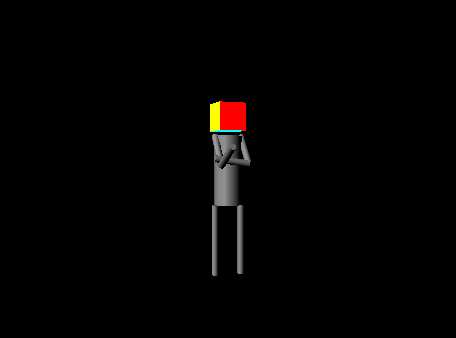
\includegraphics[width=\textwidth]{./imagenes/cortemangas-resultado.png}}
\caption{Resultado del ejemplo Corte de mangas}
\end{figure}

\end{itemize} % ends low level


\end{document}
